% \documentclass{article}
% \usepackage[utf8]{inputenc}

% \title{AProf Hw1}
% \author{André Lopes Rodrigues}
% \author{Duarte Calado Almeida}
% \date{December 2022}

% \begin{document}

% \maketitle

% \section{Introduction}

% \end{document}

\documentclass{exam}

\usepackage{titling}
\usepackage{amsmath}
\usepackage{amsfonts}
\usepackage{mathtools}
\usepackage{float}
\usepackage{tikz}
\usepackage{graphicx}
\usepackage{subfig}
\usepackage{inconsolata}
\usepackage{tikz}
\usepackage{physics}
\usepackage{amsthm}
\usepackage[font={small}]{caption}
\usepackage{courier}

\graphicspath{ {./pictures} }

\setlength{\droptitle}{-5em}   

%\renewcommand{\questionlabel}{\textbf{~\thequestion)}}
%\renewcommand{\subpartlabel}{\thesubpart)}
%\DeclarePairedDelimiterX{\norm}[1]{\lVert}{\rVert}{#1}

\newcommand*{\horzbar}{\rule[.5ex]{2.5ex}{0.5pt}}

\newenvironment{shiftedflalign*}{%
    \start@align\tw@\st@rredtrue\m@ne
    \hskip\parindent
}{%
    \endalign
}

\newcommand{\brows}[1]{%
  \begin{bmatrix}
  \begin{array}{@{\protect\rotvert\;}c@{\;\protect\rotvert}}
  #1
  \end{array}
  \end{bmatrix}
}

\newcommand{\rotvert}{\rotatebox[origin=c]{90}{$\vert$}}
\newcommand{\rowsvdots}{\multicolumn{1}{@{}c@{}}{\vdots}}

\newtheorem{lemma}{Lemma}

\title{%
  Homework 1\\
  \vspace{0.5em}
  \large Deep Learning }
\author{
  Duarte Calado de Almeida\\
  95565
  \and
  André Lopes Rodrigues\\
  96576
}
\date{}

\cfoot{\thepage}

\begin{document}
    \maketitle
    \begin{tikzpicture}[overlay, remember picture]
        \node[xshift=3.5cm,yshift=-2cm] at (current page.north west) {
\includegraphics[scale = 0.35]{logo_ist.jpg}};
    \end{tikzpicture}

    \vspace{-3em}

    \noindent\makebox[\linewidth]{\rule{18cm}{0.4pt}}

        The contribution of each member was as follows: André Rodrigues did Questions 1.1 and 2, 
        while Duarte Almeida did Questions 1.2 and 3. The elaboration of this report was made in colaboration by both students.
    % \vspace{-0.5cm}
    \noindent\makebox[\linewidth]{\rule[1ex]{18cm}{0.4pt}}
    

    \section*{Question 1}
    \begin{questions}
        \question
        \begin{parts}
            \part %1.1(a)
            After implementing the \texttt{update\_weights} method, the perceptron was trained for 20 epochs, and the validation and test accuracies were plotted as follows:
            
            \vspace{-0.4cm}
            \begin{figure}[h!]
                \centering
                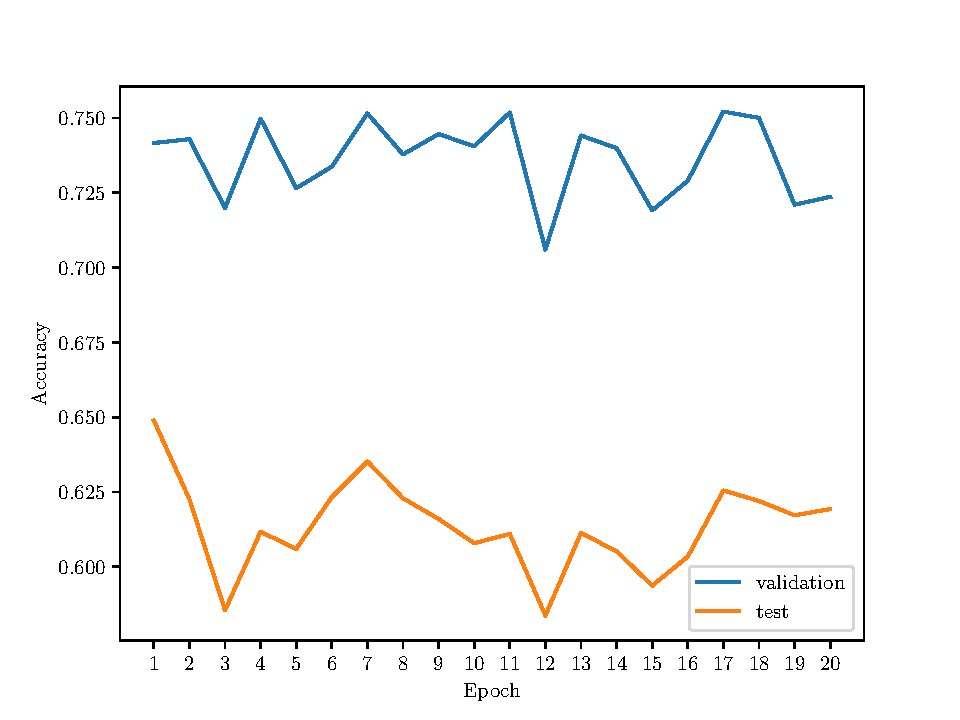
\includegraphics[scale = 0.75]{perceptron.pdf}
            \end{figure}

            The final validation and test accuracies were also obtained,
            
            \begin{table}[h!]
            \centering
                \begin{tabular}{|l|l|}
                    \hline
                    \textbf{Final Validation Accuracy} & 0.7236 \\ \hline
                    \textbf{Final Test Accuracy}       & 0.6193 \\ \hline
                \end{tabular}
            \end{table}

            \part %1.1(b)
            For the logistic regression, the corresponding \texttt{update\_weights}
            method was also obtained, and using a learning rate of $\eta = 0.001$,
            the model was trained for 20 epochs, having the accuracies for the validation
            and test set also been plotted:
            
            \begin{figure}[H]
                \centering
                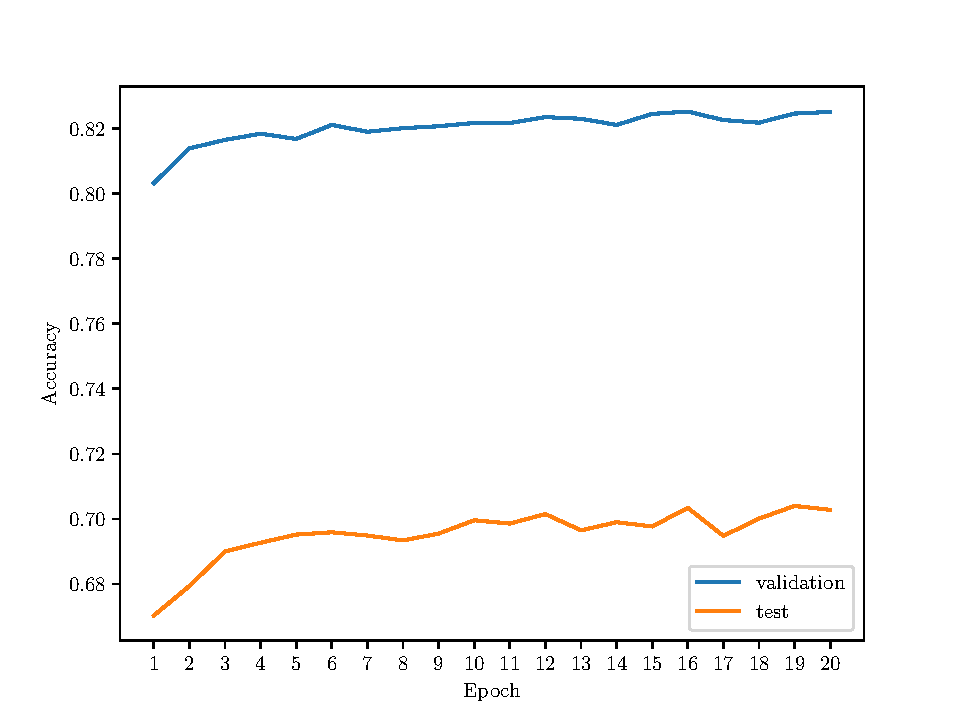
\includegraphics[scale = 0.75]{logistic_regression.pdf}
            \end{figure}
            % \begin{align*}
            %     \text{Final accuracy on validation set: } 0.8251 \\
            %     \text{Final accuracy on test set: } 0.7028
            % \end{align*}
            The final validation and test accuracies obtained are as follows,
            \begin{table}[h!]
            \centering
                \begin{tabular}{|c|c|}
                    \hline
                    \textbf{Final Validation Accuracy} & 0.8251 \\ \hline
                    \textbf{Final Test Accuracy}       & 0.7028 \\ \hline
                \end{tabular}
            \end{table}
            
        \end{parts}
        %\newpage
        \question
        \begin{parts}
            %1.2(a)
            \part The use of multilayer perceptrons provides a form of \textbf{representation learning} through the composition of multiclass perceptrons with non-linear activation functions; in particular, they are able to search through some subspace of feature transformations and find one for which the linear separation of data is easier. In practical terms, this layering provides \textbf{hierarchical compositionality}, i.e., each layer encodes a distributed representation that is more abstract the closer it is to the output layer, finding meaningful features at different levels of granularity. \\
            In the context of character recognition, MLPs are usually able to successively detect features of symbols (i.e., edges and parts), combine them in coarser features and perform an accurate classification at the end. This is usually not the case if we use simple perceptrons, as plain linear combinations of grayscale values are less capable of detecting those distinctive features and of being flexible to the variability that the same character may show.\\
            Nevertheless, an MLP that \textbf{only} uses linear activation functions ($g(z) = z$) \textbf{does not display this feature}, as it corresponds to a linear classifier, effectively functioning like a simple perceptron:
            \begin{align*}
                \vb*{f}(\vb*{x})&= g(\vb*{z}^{(L + 1)}) = \vb*{z}^{(L + 1)} \\
                &= \vb*{W}^{(L + 1)}\vb*{h}^{(L)} + \vb*{b}^{(L + 1)} \\
                &= \vb*{W}^{(L + 1)}(\vb*{W}^{(L)}\vb*{h}^{(L - 1)} + \vb*{b}^{(L)}) + \vb*{b}^{(L + 1)} \\
                & \qquad \qquad \dots\\
                &= \vb*{W}^{(L + 1)}(\vb*{W}^{(L)}( \dots \; (\vb*{W}^{(1)}\vb*{x} + \vb*{b}^{(1)}))+ \vb*{b}^{(L)}) + \vb*{b}^{(L + 1)} \\
                &=  \underbrace{\vb*{W}^{(L + 1)} \dots  \vb*{W}^{(1)}}_{\vb*{\widetilde{W}}} \vb*{x} + \underbrace{\vb*{W}^{(L + 1)} \dots \vb*{W}^{(2)} \vb*{b}^{(1)} + \dots + \vb*{W}^{(L + 1)} \vb*{b}^{(L)} + \vb*{b}^{(L + 1)}}_{\vb*{\widetilde{b}}}
            \end{align*}
            \newpage
            %1.2(b)
            \part
            Having implemented the code for the multi-layer perceptron (with a single hidden layer) and its backpropagation algorithm, the model was built with 200 hidden units, \textbf{\texttt{ReLU}} as the activation function, and cross-entropy as the loss criterion. 
            Stochastic gradient descent was then used to train the model for 20 epochs, with a learning rate of $\eta = 0.001$. The weights were initialized with a normal distribution $w_{ij} \sim \mathcal{N}(\mu, \sigma^2)$, with mean $\mu = 0.1$ and variance $\sigma^2 = 0.1$ and bias set to zero. The accuracies for the validation and test sets were then plotted:
            \vspace{-0.4cm}
            \begin{figure}[h!]
                \centering
                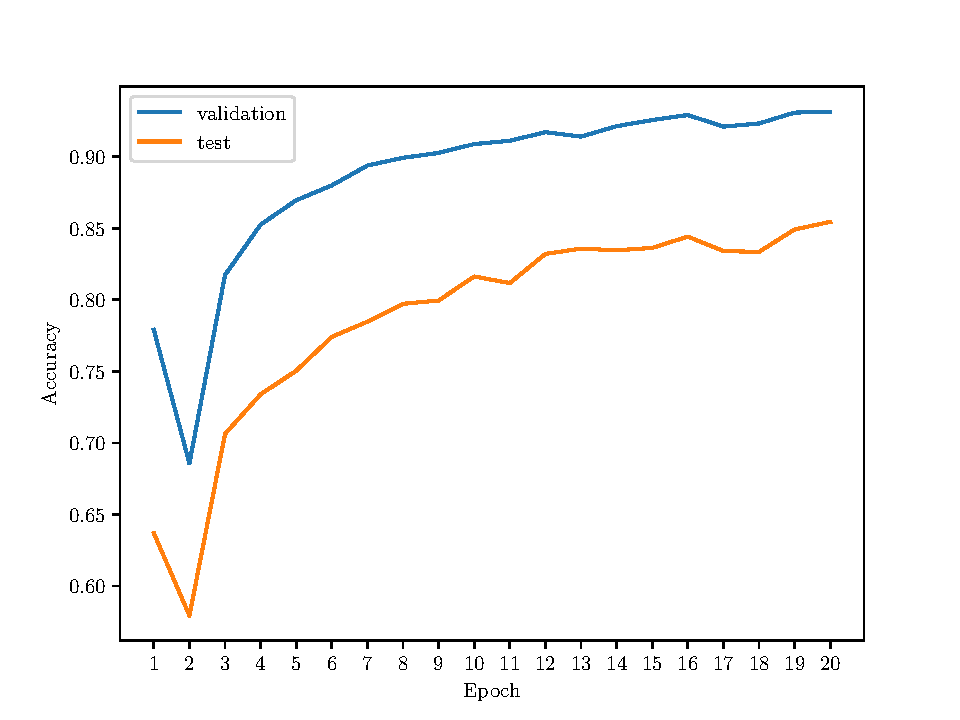
\includegraphics[scale = 0.75]{mlp.pdf}
            \end{figure}

            The final validation and test accuracies were also obtained,  
            
            \begin{table}[h!]
            \centering
                \begin{tabular}{|c|c|}
                    \hline
                    \textbf{Final Validation Accuracy} & 0.9316 \\ \hline
                    \textbf{Final Test Accuracy}       & 0.8545 \\ \hline
                \end{tabular}
            \end{table}
            
            % \begin{align*}
            %     \text{Final accuracy on validation set: } 0.9316 \\
            %     \text{Final accuracy on test set: } 0.8545
            % \end{align*}
            
            

        \end{parts}

    \end{questions}

    \section*{Question 2}

    \begin{questions}
        \question %2.1
        For the linear model with logistic regression, the best configuration in terms of \textbf{validation accuracy} is the one with 
 a learning rate of $\eta = \textbf{0.001}$, as shown in the table below. The final \textbf{test error} in that configuration is 0.7019.
        
        \begin{table}[h!]
            \centering
            \begin{tabular}{c|ccccc}
                                &                                     & learning rate                      &                 &  &  \\ \cline{2-4}
                                & \multicolumn{1}{c|}{0.001}          & \multicolumn{1}{c|}{0.01}          & 0.1             &  &  \\ \cline{1-4}
            validation accuracy & \multicolumn{1}{c|}{0.8256} & \multicolumn{1}{c|}{0.8033} & 0.7516 &  & 
            \end{tabular}
        \end{table}

    \newpage

        The plots of the loss and validation accuracy over the number of epochs, respectively, for the learning rate of $\eta = 0.001$ can be found below.

        \begin{figure}[H]
            \centering
            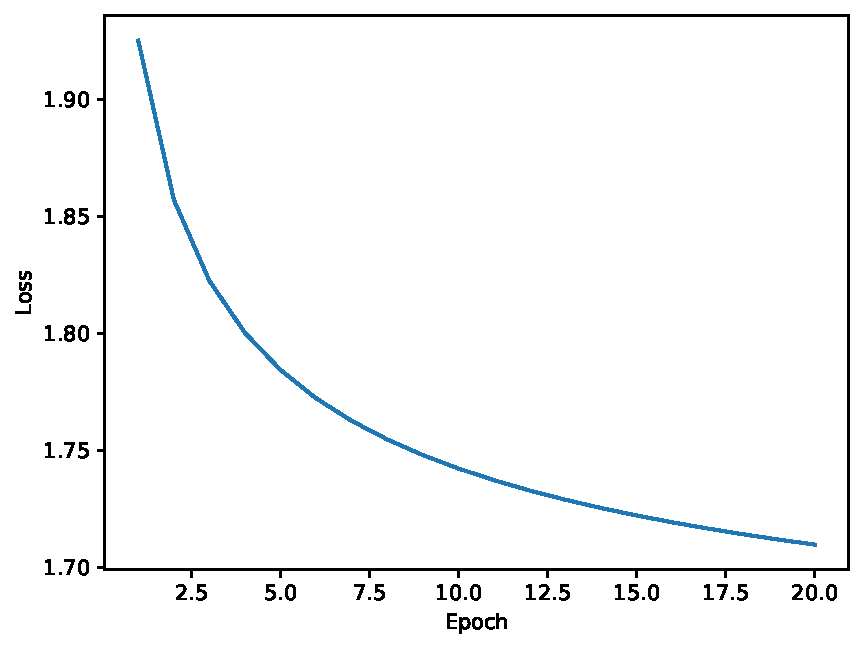
\includegraphics[scale = 0.75]{logistic_regression-training-loss-0.001-sgd.pdf}
        \end{figure}

        \begin{figure}[H]
            \centering
            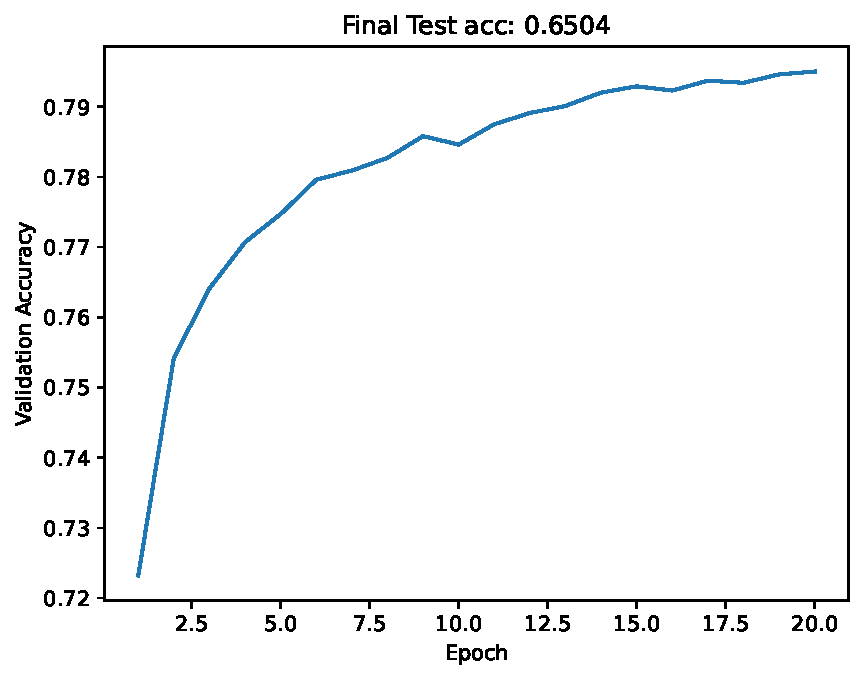
\includegraphics[scale = 0.75]{logistic_regression-validation-accuracy-0.001-sgd.pdf}
        \end{figure}

        \question %2.2
        The best configuration for the feedforward neural network in terms of \textbf{validation accuracy}
        is the one that maintains the default configuration but that uses \textbf{200 hidden units}, 
        as shown in the table below. The final \textbf{test error} in that configuration is 0.8820.
        %0.8619, 0.7429||   (0.9431, 0.8674) ||  (0.9535, 0.8932)
        \begin{table}[h!]
            \centering
            \begin{tabular}{c|ccc|cc|cc|cc}
                                & \multicolumn{3}{c|}{learning rate}                            & \multicolumn{2}{c|}{hidden size} & \multicolumn{2}{c|}{dropout}     & \multicolumn{2}{c}{activation}   \\ \cline{2-10} 
                                & \multicolumn{1}{c|}{0.001} & \multicolumn{1}{c|}{0.01} & 0.1  & \multicolumn{1}{c|}{100}  & 200  & \multicolumn{1}{c|}{0.3}  & 0.5  & \multicolumn{1}{c|}{relu} & tanh \\ \hline
            validation accuracy & \multicolumn{1}{c|}{0.8658} & \multicolumn{1}{c|}{0.9391} & 0.9439 & \multicolumn{1}{c|}{0.9391} & 0.9490 & \multicolumn{1}{c|}{0.9391} & 0.9312 & \multicolumn{1}{c|}{0.9391} & 0.9140
            \end{tabular}
        \end{table}
        
        \newpage

        Below are the plots for respectively, the loss and the validation accuracy over the number of epochs,
        for 200 hidden units:

        \begin{figure}[H]
            \centering
            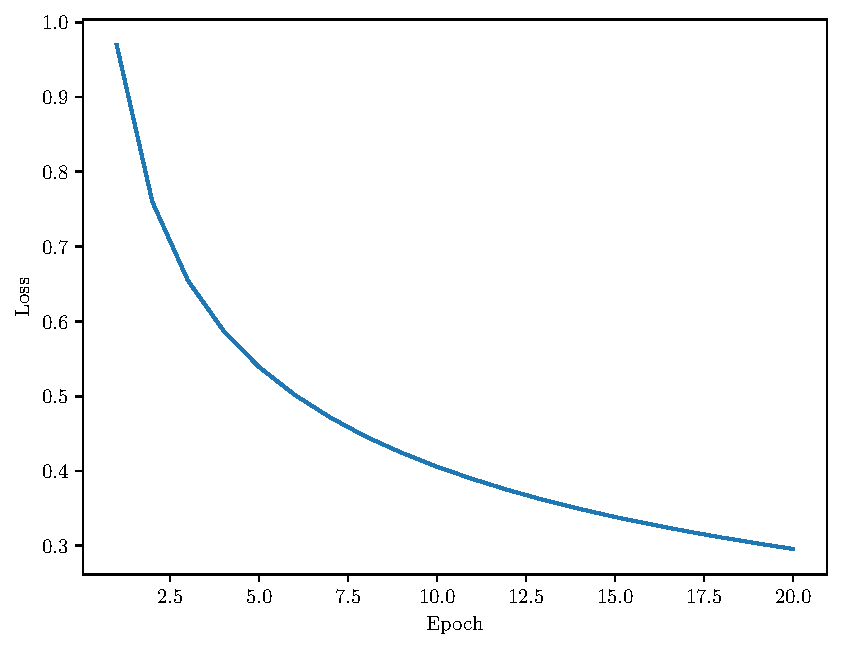
\includegraphics[scale = 0.75]{feedforward-training-loss-0.01-200-1-0.3-relu-sgd-16.pdf}
        \end{figure}

        \begin{figure}[H]
            \centering
            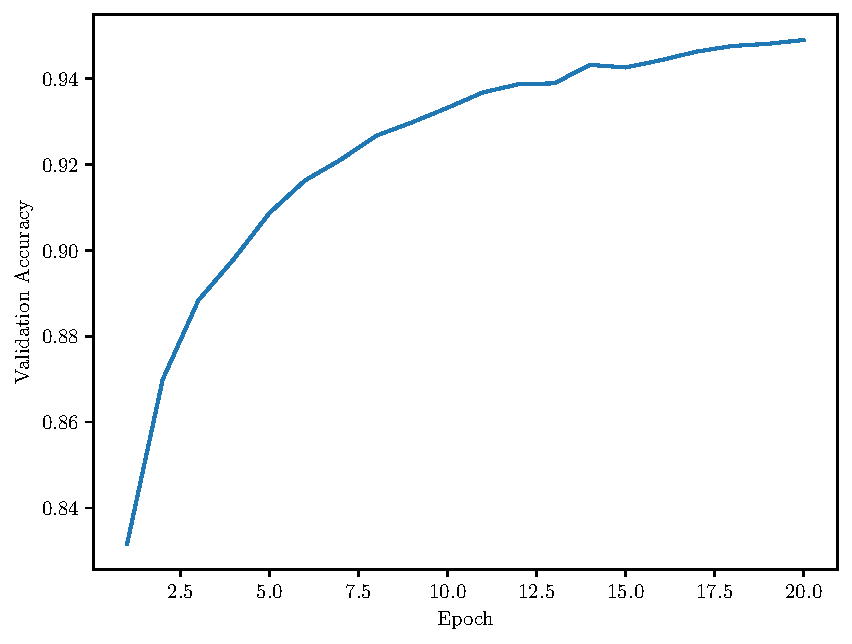
\includegraphics[scale = 0.75]{feedforward-validation-accuracy-0.01-200-1-0.3-relu-sgd-16.pdf}
        \end{figure}
        \question %2.3

        Using the default hyperparameters, the number of hidden layers was increased
        and it was found that the best configuration in terms of \textbf{validation accuracy} is the one with \textbf{2 hidden layers},
        as shown in the table below. The final \textbf{test error} in that configuration is 0.8707.

        \begin{table}[h!]
            \centering
            \begin{tabular}{l|cc}
                 & \multicolumn{2}{c}{hidden layers}     \\ \cline{2-3} 
                 & \multicolumn{1}{c|}{2}      & 3       \\ \hline
                    \multicolumn{1}{c|}{validation accuracy} & \multicolumn{1}{c|}{0.9448} & 0.9407
            \end{tabular}
        \end{table}

        The plots of the loss and validation accuracy of the model with 2 hidden layers are as follows,

        \begin{figure}[H]
            \centering
            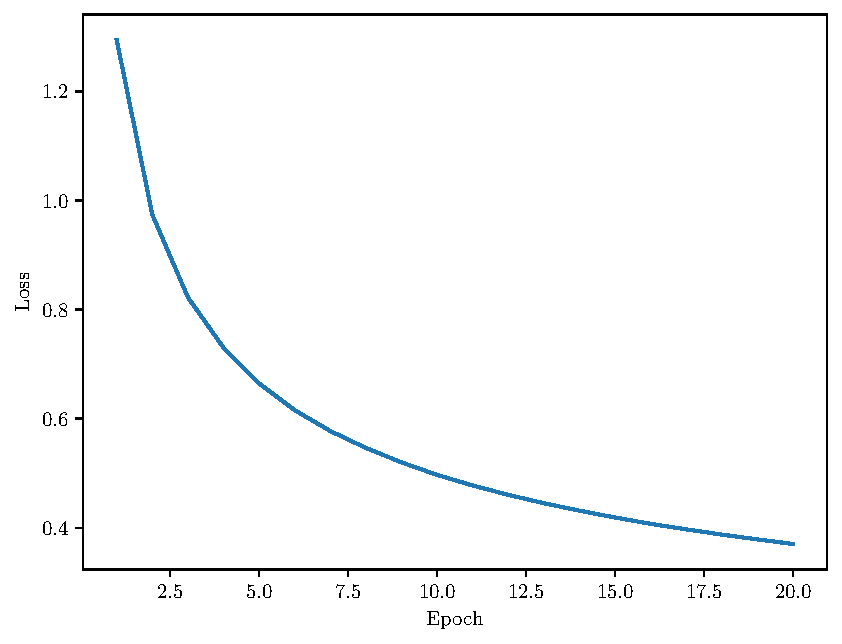
\includegraphics[scale = 0.75]{feedforward-training-loss-0.01-100-2-0.3-relu-sgd-16.pdf}
        \end{figure}
    
        \begin{figure}[H]
            \centering
            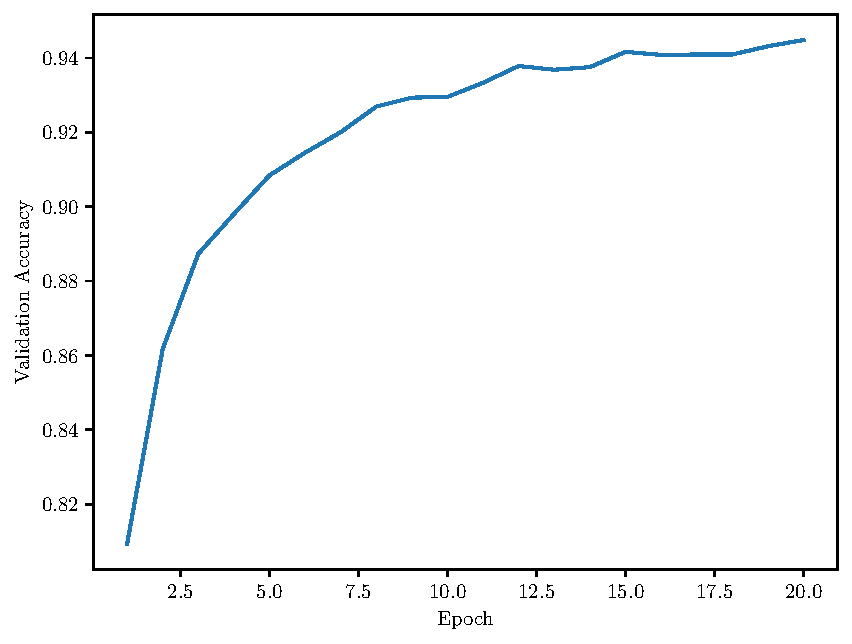
\includegraphics[scale = 0.75]{feedforward-validation-accuracy-0.01-100-2-0.3-relu-sgd-16.pdf}
        \end{figure}

    \end{questions}

    \newpage

    \section*{Question 3}
    \begin{questions}
        \question
        Let $x_i$ denote the $i$-th component of $\vb*{x}$ and let $w_{ij}$ denote the entry in the $i$-th row and $j$-th column in matrix $\vb*{W}$. We then have that:

        \begin{align*}
            h_i(\vb*{x}) &= g\left(\sum_{j = 1}^{D} w_{ij}x_j \right) = \left(\sum_{j = 1}^{D} w_{ij}x_j \right)^2 = \left(\sum_{j = 1}^{D} w_{ij}x_j\right)\left( \sum_{k = 1}^{D} w_{ik}x_k\right) \\
            &= \sum_{j = 1}^{D} \sum_{k = 1}^{D} w_{ij}x_j  w_{ik}x_k = \sum_{j = 1}^{D} w_{ij}^2x_j^2 +  \sum_{j = 1}^{D} \sum_{k \neq j} w_{ij}w_{ik}x_j x_k \\
            &= \sum_{j = 1}^{D} w_{ij}^2x_j^2 + \sum_{j = 1}^{D} \sum_{k = 1}^{j - 1}  w_{ij}w_{ik}x_j x_k + 
            \sum_{j = 1}^{D} \sum_{k = j + 1}^{D}  w_{ij}w_{ik}x_j x_k \\
            &= \sum_{j = 1}^{D} w_{ij}^2x_j^2 +\sum_{k = 1}^{D} \sum_{j = k + 1}^{D}  w_{ij}w_{ik}x_j x_k + 
            \sum_{j = 1}^{D} \sum_{k = j + 1}^{D}  w_{ij}w_{ik}x_j x_k \\
            &= \sum_{j = 1}^{D} w_{ij}^2x_j^2 + \sum_{k = 1}^{D} \sum_{j = k + 1}^{D} w_{ij}w_{ik}(2x_j x_k) \\
            &= 
            \begin{bmatrix}
                w_{i1}^2 & w_{i1}w_{i2} & \dots & w_{i1}w_{iD} & w_{i2}^2 & w_{i2}w_{i3} & \dots & w_{i(D - 1)}^2  & w_{i(D - 1)} w_{iD} &  w_{iD}^2
            \end{bmatrix}
            \begin{bmatrix}
                x_1^2 \\ 2x_1 x_2 \\ \dots \\ 2x_1 x_D \\ x_2^2 \\ 2x_2 x_3 \\ \dots \\ x_{D - 1}^2 \\ 2x_{D - 1} x_{D} \\  x_{D}^2
            \end{bmatrix}
        \end{align*}
        As such, $\vb*{h}$ is linear in some feature transformation $\vb*{\phi}$, that is, $\vb*{h}$ can be written as $\vb*{A}_{\Theta}\vb*{\phi}(\vb*{x})$. In particular, we have that such matrix $\vb*{A}_{\Theta}$ can be defined as:
        \begin{equation*}
            \vb*{A}_{\Theta} = 
            \brows{\vb*{a}_1^T \\ \vb*{a}_2^T \\ \rowsvdots \\ \vb*{a}_K^T}
        \end{equation*}
        where
        \begin{equation*}
            \vb*{a}_i = 
            \begin{bmatrix}
            w_{i1}^2 & w_{i1}w_{i2} & \dots & w_{i1}w_{iD} & w_{i2}^2 & w_{i2}w_{i3} & \dots & w_{i(D - 1)}^2  & w_{i(D - 1)} w_{iD} &  w_{iD}^2
            \end{bmatrix}^T
        \end{equation*}
        and so $\vb*{A}_{\Theta} \in \mathbb{R}^{K \times \frac{D(D + 1)}{2}}$ (since $\sum_{k = 1}^{D} k = \frac{D(D + 1)}{2}$). Furthermore, we can define the feature transformation $\vb*{\phi} : \mathbb{R}^D \mapsto  \mathbb{R}^{\frac{D(D + 1)}{2}}$ as:
        \begin{equation*}
            \vb*{\phi}(\vb*{x}) = (x_1^2, 2x_1 x_2, \dots, 2x_1 x_D, x_2^2, 2x_2 x_3, \dots, x_{D - 1}^2, 2x_{D - 1} x_{D}, x_{D}^2)
        \end{equation*}

        \question
        Given that the predicted output $\hat{y}$ is defined as:
        \[
            \hat{y} = \vb*{v}^T \vb*{h}
        \]
        the linearity of $\vb*{h}$ in the feature transformation $\vb*{\phi}(\vb*{x})$ proven above leads to the following equality:
        \[
            \hat{y} = \vb*{v}^T \vb*{A}_{\Theta} \vb*{\phi}(\vb*{x}) 
                    = (\vb*{A}_{\Theta}^T \vb*{v})^T \vb*{\phi}(\vb*{x}) 
                    = \vb*{c}_{\Theta}^T \vb*{\phi}(\vb*{x}) 
        \]
        where we take $\vb*{c}_{\Theta}$ to be equal to $\vb*{A}_{\Theta}^T \vb*{v}$, thereby proving that $\hat{y}$ is also a linear transformation of $\vb*{\phi}(\vb*{x})$. However, $\hat{y}$ is \textbf{not} linear in terms of the original parameters $\Theta$. To see this, note that the model is now a linear combination of \textbf{products} of entries of $\vb*{W}$ and $\vb*{v}$ rather than being linear in \textbf{each} individual entry:
        \[
            \hat{y} = \vb*{v}^T \vb*{A}_{\Theta} \vb*{\phi}(\vb*{x}) = \sum_{i = 1}^{D} v_i (\vb*{w}_i^T \vb*{x})^2 
            = \sum_{i = 1}^{K} \sum_{j = 1}^{D} \sum_{k = 1}^{D} v_i w_{ij} w_{ik} x_i x_k
        \]
        where we define $\vb*{w}_i$ to be the vector in the $i$-th row of matrix $\vb*{W}$.

        \question
        \begin{proof}[\unskip\nopunct]
        To prove the desired result, for $\vb*{c}_{\Theta}$ defined in the previous subquestion and for any $\vb*{c} \in \mathbb{R}^{\frac{D(D + 1)}{2}}$, we make the observation that the inner products $\vb*{c}_{\Theta}^T  \vb*{\phi}(\vb*{x})$ and $\vb*{c}^T  \vb*{\phi}(\vb*{x})$ actually correspond to quadratic forms in $\vb*{x}$:
        \begin{align*}
            \vb*{c}_{\Theta}^T \vb*{\phi(x)} &= \vb*{v}^T \vb*{h} = \sum_{i = 1}^K v_i (\vb*{A}_{\Theta} \vb*{\phi}(\vb*{x}))^2_i = 
            \sum_{i = 1}^K v_i (\vb*{w}_i^T \vb*{x})^2 \\
            &= 
            \begin{bmatrix}
                \vb*{w}_1^T \vb*{x} & \vb*{w}_2^T \vb*{x} & \dots & \vb*{w}_K^T \vb*{x}
            \end{bmatrix}
            \text{diag}(\vb*{v})
            \begin{bmatrix}
                \vb*{w}_1^T \vb*{x} \\ \vb*{w}_2^T \vb*{x} \\ \dots \\ \vb*{w}_K^T \vb*{x}
            \end{bmatrix} \\
            &= (\vb*{Wx})^T \text{diag}(\vb*{v}) \vb*{Wx} 
             = \vb*{x}^T \vb*{W}^T \text{diag}(\vb*{v}) \vb*{Wx} 
        \end{align*}
        and 
        \begin{align*}
            \vb*{c}^T \vb*{\phi(x)} &= \sum_{i = 1}^{\frac{D(D + 1)}{2}} c_i \phi_i(x) = \sum_{i = 1}^{D} c_{(i - 1)D + i - \frac{(i - 1)i}{2}}\; x_i^2 + \sum_{i = 1}^{D}\sum_{j = i + 1}^{D} c_{(i - 1)D + j - \frac{(i - 1)i}{2}}\;(2 x_i x_j) \\
            &= \vb*{x}^T \mathcal{M}(\vb*{c}) \vb*{x}
        \end{align*}
        where $\mathcal{M}(\vb*{c}) \in \mathbb{R}^{D \times D}$ is a symmetric matrix obtained from $\vb*{c}$ such that:
        \begin{itemize}
            \item[--] the diagonal and the part above the diagonal of the matrix $\mathcal{M}(\vb*{c})$ are filled row-wise with the elements of vector $\vb*{c}$, i.e.:
            \[
                \mathcal{M}(\vb*{c}) = 
                \begin{bmatrix}
                    c_1 & c_2 & c_3 & \dots & c_D \\
                    c_2 & c_{D + 1} & c_{D + 2} & \dots & c_{2D - 1} \\
                    \vdots & \vdots & \vdots & \ddots & \vdots \\
                    c_D & c_{D - 1} & c_{D - 2} & \dots & c_{\frac{D(D + 1)}{2}} 
                \end{bmatrix}
            \]
            \item[--] for $1 \le i \le D$ and $j < i$, $(\mathcal{M}(\vb*{c}))_{ij} = (\mathcal{M}(\vb*{c}))_{ji}$
        \end{itemize}
        Furthermore, we also recur to the following lemma:

        \begin{lemma}
            Two vectors $\vb*{a}, \: \vb*{b} \in \mathbb{R}^{\frac{D(D + 1)}{2}}$ are equal if and only if $\vb*{a}^T \vb*{\phi(x)} = \vb*{b}^T \vb*{\phi(x)}$, for all $\vb*{x} \in \mathbb{R}^D$
        \end{lemma}
        \begin{proof}
            If $\vb*{a} = \vb*{b}$, then $\vb*{a}^T \vb*{\phi(x)} = \vb*{b}^T \vb*{\phi(x)}$ is trivially verified. For the reverse implication, note that, according to the previously made observation, for any $\vb*{x} \in \mathbb{R}^D$:
            \[
                \vb*{a}^T \vb*{\phi(x)} = \vb*{b}^T \vb*{\phi(x)} \Rightarrow \vb*{x}^T \mathcal{M}(\vb*{a}) \vb*{x} = \vb*{x}^T \mathcal{M}(\vb*{b}) \vb*{x}
            \]
            Since both $\mathcal{M}(\vb*{a})$ and $\mathcal{M}(\vb*{a})$ are symmetric and the associated quadratic forms are twice continuously differentiable, taking the hessian on both sides of the equation yields:
            \[
                \mathcal{M}(\vb*{a}) = \mathcal{M}(\vb*{b})
            \]
            that is, $\mathcal{M}(\vb*{a})$ and $\mathcal{M}(\vb*{b})$ are equal entry-wise. In particular, we have that $a_i = b_i$, for $i = 1, \dots, \frac{D(D + 1)}{2}$.
        \end{proof}
        We are now equipped with the tools needed for the proof. Since $\mathcal{M}(\vb*{c})$ is symmetric, the \textbf{Spectral Decomposition Theorem} tells us that there is an orthonormal matrix $\vb*{Q}$ and a diagonal matrix $\vb*{\Lambda}$ such that $\mathcal{M}(\vb*{c}) = \vb*{Q} \vb*{\Lambda}\vb*{Q}^T$. Let $\vb*{q_i}$ denote the eigenvector of $\mathcal{M}(\vb*{c})$ that is present in $i$-th column of $\vb*{Q}$ and let $\lambda_i$ be the corresponding eigenvalue (note that $\{\vb*{q}_i\}_{i = 1}^{D}$ forms an orthonormal basis of $\mathbb{R}^{D}$). Then, we can write $\vb*{c}^T \vb*{\phi(x)}$ as:
        \[
            \vb*{c}^T \vb*{\phi(x)} =  \vb*{x}^T \mathcal{M}(\vb*{c}) \vb*{x} = (\vb*{Q}^T \vb*{x})^T \vb*{\Lambda} (\vb*{Q}^T \vb*{x}) = \sum_{i = 1}^{D} \lambda_i (\vb*{q}_i^T\vb*{x})^2
        \]
        Now, if we assume that $K \ge D$, we can find a matrix $\vb*{W}$ and a vector $\vb*{v}$ that make $\vb*{c}^T_{\Theta} \vb*{\phi(x)}$ equal to $\vb*{c}^T \vb*{\phi(x)}$ in the following way:
        \begin{itemize}
            \item[--] we make $\vb*{v}$ to be equal to $(\lambda_1, \lambda_2, \dots, \lambda_D, \underbrace{0, \dots, 0}_{K - D \: \text{times}})$;
            \item[--] we make $\vb*{W}$ to be equal to the vertical concatenation of $\vb*{Q}^T$ with a $(K - D) \times D$ matrix of zeros, i.e.:
            \begin{align*}
            \vb*{W} = 
                \begin{bmatrix}
                    &\vb*{Q}^T \\
                    &\vb*{0}_{(K - D) \times D}
                \end{bmatrix}
            \end{align*}
        \end{itemize}
        We then have that:
        \[
            \vb*{c}^T_{\Theta} \vb*{\phi(x)} = \sum_{i = 1}^{K} v_i (\vb*{w}_i^T\vb*{x})^2 =  \sum_{i = 1}^{D} \lambda_i (\vb*{q}_i^T\vb*{x})^2 = (\vb*{Q}^T \vb*{x})^T \vb*{\Lambda} (\vb*{Q}^T \vb*{x}) = \vb*{x}^T \vb*{Q} \vb*{\Lambda}\vb*{Q}^T \vb*{x} = \vb*{c}^T \vb*{\phi(x)}
        \]
        and, by Lemma 1, we prove that the previous choice of $\vb*{W}$ and $\vb*{v}$ originates a vector $\vb*{c}_{\Theta}$ such that $\vb*{c}_{\Theta} = \vb*{c}$. Furthermore, we have proven that the sets of classifiers $\mathcal{C}_1 = \{\vb*{c}_{\Theta}^T\vb*{\phi(x)} : \Theta = (\vb*{W}, \vb*{v}) \in \mathbb{R}^{K \times D \times K}\}$ and $\mathcal{C}_2 = \{\vb*{c}^T\vb*{\phi(x)} : \vb*{c} \in \mathbb{R}^{\frac{D(D + 1)}{2}}\}$ are exactly the same, and so the original neural network reduces to a \textbf{linear model} in terms of $\vb*{c}_{\Theta}$.
        \end{proof}
 
        Consider now the case when $K < D$. Then, the nullspace of $\vb*{W}$ has at least dimension $D - K \ge 1$, and thus there is some \textbf{non-null} vector $\vb*{x^*}$ such that $\vb*{Wx^*} = 0$. Now, choose $\vb*{c}$ to be a vector such that $\mathcal{M}(\vb*{c}) = \vb*{I}_{D \times D}$ (i.e., the $D \times D$ identity matrix). We then have:
        \[
            \vb*{c}^T_{\Theta} \vb*{\phi(x^*)}
            = \vb*{x^*}^T \vb*{W}^T \text{diag}(\vb*{v}) \vb*{Wx^*} = 0
        \]
        and
        \[
            \vb*{c}^T \vb*{\phi(x^*)} = \vb*{x^*}^T \mathcal{M}(\vb*{c}) \vb*{x^*} = \vb*{x^*}^T \vb*{I}_{D \times D} \vb*{x^*} = \|\vb*{x^*}\|_2^2 > 0 
        \]
        Thus, for $K < D$, we have constructed an instance of $\vb*{c}$ for which there exists some $\vb*{x} \in \mathbb{R}^{D}$ such that  $\vb*{c}^T_{\Theta} \vb*{\phi(x)} \neq \vb*{c}^T \vb*{\phi(x)}$. Applying Lemma 1, we conclude that there is no choice of parameters $\vb*{W}$ and $\vb*{v}$ that make $\vb*{c}_{\Theta}$ equal to $\vb*{c}$ and so the model cannot be parametrized by $\vb*{c}_{\Theta}$ in this case.

        \question
        Given that $\hat{y} = \vb*{c}^T_{\Theta} \vb*{\phi}(\vb*{x})$, we can write the squared loss as:
        \[
            L(\vb*{c}^T_{\Theta}; \mathcal{D}) = \frac{1}{2} \sum_{n = 1}^{N} (\hat{y}_n(\vb*{x}_n; \vb*{c}^T_{\Theta}) - y_n) ^2 = \frac{1}{2} \sum_{n = 1}^{N} (\vb*{c}^T_{\Theta} \vb*{\phi}(\vb*{x}) - y_n) ^2 = \frac{1}{2} \|\vb*{X}\vb*{c}_{\Theta} - \vb*{y} \|_2^2
        \]
        where $\vb*{y} = (y_1, y_2, \dots, y_n)$. As such, the minimization of the squared lost corresponds to a linear least squares problem, which in this case has a unique solution $\vb*{c}^*_{\Theta}$ that is found simply by setting the gradient to zero:
        \begin{align*}
            \nabla_{\vb*{c}_{\Theta}} L(\vb*{c}^T_{\Theta}; \mathcal{D}) = \vb*{0} &\Leftrightarrow \nabla_{\vb*{c}_{\Theta}}(\vb*{X}\vb*{c}_{\Theta}) \nabla_{\vb*{z}}\left(\frac{1}{2}\|\vb*{z}\|_2^2\right) \rvert_{\vb*{z} = \vb*{X}\vb*{c}_{\Theta} - \vb*{y}} = \vb*{0} \Leftrightarrow \vb*{X}^T(\vb*{X}\vb*{c}_{\Theta} - \vb*{y}) = \vb*{0} \\
            &\Rightarrow \vb*{c}^*_{\Theta} = (\vb*{X}^T\vb*{X})^{-1}\vb*{X}^T\vb*{y}
        \end{align*}
        To prove the existence of $ (\vb*{X}^T\vb*{X})^{-1}$, note that the dimensions of the nullspaces of and $\vb*{X}$ and $\vb*{X}^T\vb*{X}$ are equal, since, for every $\vb*{x} \in \mathbb{R}^{\frac{D(D + 1)}{2}}$:
        \[
            \vb*{X}\vb*{x} = \vb*{0} \Rightarrow \vb*{X}^T\vb*{X}\vb*{x} = \vb*{0}
        \]
        and 
        \[
            \vb*{X}^T\vb*{X}\vb*{x} = \vb*{0} \Rightarrow \vb*{x}^T\vb*{X}^T\vb*{X}\vb*{x} = \vb*{0} 
            \Rightarrow \|\vb*{X}\vb*{x}\|_2^2 = \vb*{0} \Rightarrow \vb*{X}\vb*{x} = \vb*{0}
        \]
        Since $N > \frac{D(D + 1)}{2}$ and $\vb*{X}$ has full column rank ($\frac{D(D + 1)}{2}$), its nullspace has dimension $0$. Hence, $\vb*{X}^T\vb*{X}$ is a $\frac{D(D + 1)}{2} \times \frac{D(D + 1)}{2}$ square matrix with rank $\frac{D(D + 1)}{2} - 0 = \frac{D(D + 1)}{2}$, and so it is invertible. \par
        Usually, loss functions of feedforward neural networks are non-convex in their parameters due to multiple compositions of non-linear activation functions, making the global minimization of said functions especially hard. In spite of that, since the presented architecture only has a single hidden layer with at least as many units as the input layer and uses only quadratic activations, we managed to reduce it to a \textbf{linear regression} by defining the underlying \textbf{feature transformation} $\vb*{\phi}$ and \textbf{weight vector} $\vb*{c}_{\Theta}$. Hence, the minimization of the loss function becomes much easier, since the global minimizer can be computed in closed form.
    \end{questions}
\end{document}